\documentclass[]{article}

\begin{document}

\section{Mockups}
\label{Mockups}
\subsection{Menubalk}
In de menubalk van de applicatie vindt de gebruiker onder Bestand de mogelijkheid terug om een programma op te slaan, in te laden of om een nieuw programma te maken. Bij instellingen kan hij de console aan en uitzetten en de taal van de applicatie veranderen.\\In het midden van de menubalk vinden we een start knop waarmee de uitvoering van het programma wordt gestart mits het correct geconstrueerd is. Hiernaast bevindt zich ook de knop om de uitvoering te stoppen.\\ Aan de rechterzijde bevindt zich een switch bestaande uit drie knoppen: Klasse, Kabels en Events. Deze stellen de verschillende delen van de IDE voor die gebruikt worden om een programma te cree\"{e}ren. De beschrijving van deze delen op hoog niveau staat in Sectie \ref{interpretatie}.
\subsection{Klasse creatie}

Bij het selecteren van Klasse in de switch zal aan de gebruiker het klasse creatie view getoond worden. De mockup van dit view is te zien op figuur \ref{creatieklassemockup}. Hierin vindt hij onder de menubalk een balk waarin de reeds gecree\"{e}rde klasse zich als tabbladen bevindt. Op het einde van deze balk bevindt er zich een plus toets waarmee een nieuwe klasse kan worden toegevoegd.\\\\Aan de linkerzijde vindt de gebruiker alle categorie\"{e}n van de programmeerblokken. Bij het selecteren van een categorie zullen alle blokken die tot die categorie behoren verschijnen onder de categorie\"{e}n. Bij het aanklikken van een blok zal deze op het creatie veld verschijnen.\\\\ De kleuren en vorm van blokken, types en events moet nog aangepast worden op het eenvoudige gebruik van de applicatie en het proffesionele uitzicht ervan. Onderstaande mockups dienen voor het aantonen van de werking van de applicatie.\\ Het inelkaar klikken van blokken zal op een intu\"{i}tieve manier moeten duidelijk worden gemaakt. Als een blok de andere niet accepteerd zal deze er boven op blijven zweven maar zal het voor de gebruiker duidelijk zijn dat de blokken niet verbonden zijn.\\\\ Het verbinden van input events met de handler die de gebruiker wenst gebeurt met pijlen. Hierbij zal een pijl enkel kunnen verbonden worden als de handler ook het juiste event als input parameter heeft.\\ Het definieren van een functie gebeurt doormiddel van een functieblok. Deze kan de gebruiker een naam geven. Voor het toevoegen van een parameter moet de gebruiker op plus tekenen duwen en een variable en een type invullen. Het oproepen van een functie kan met een functiecallblok. Deze bestaat uit een blokje waaraan een pijl zit met een andere blok waarin de gebruiker een functie kan selecteren uit een lijst van functies uit die klasse. Onderaan dit blok kan een blokje staan waarin de return waarde van de functie kan worden opgevangen.\\\\ Aan de rechterzijde van de klasse creatie bevinden zich alle uitlijken van die tot een klasse behoren. Zo kan een klasse lamp bijvoorbeeld twee uitlijken bezitten namelijk een uit en aan afbeelding. Deze kan dan worden veranderd door een verander van uiterlijk blok.\\Hieronder bevinden zich de member variable van de klasse. Deze kan de gebruiker aanmaken door op het plus teken te drukken en een variabele van het gewenste type aan te maken met een unieke naam. Hiervan kunnen dan blokken op het creatie veld worden geplaats om te gebruiken in functies of handlers. Tenslotte vind de gebruiker hieronder alle events die hij reeds gedefineerd heeft in de event sectie van de IDE. 


 \begin{sidewaysfigure}
  \centering
   
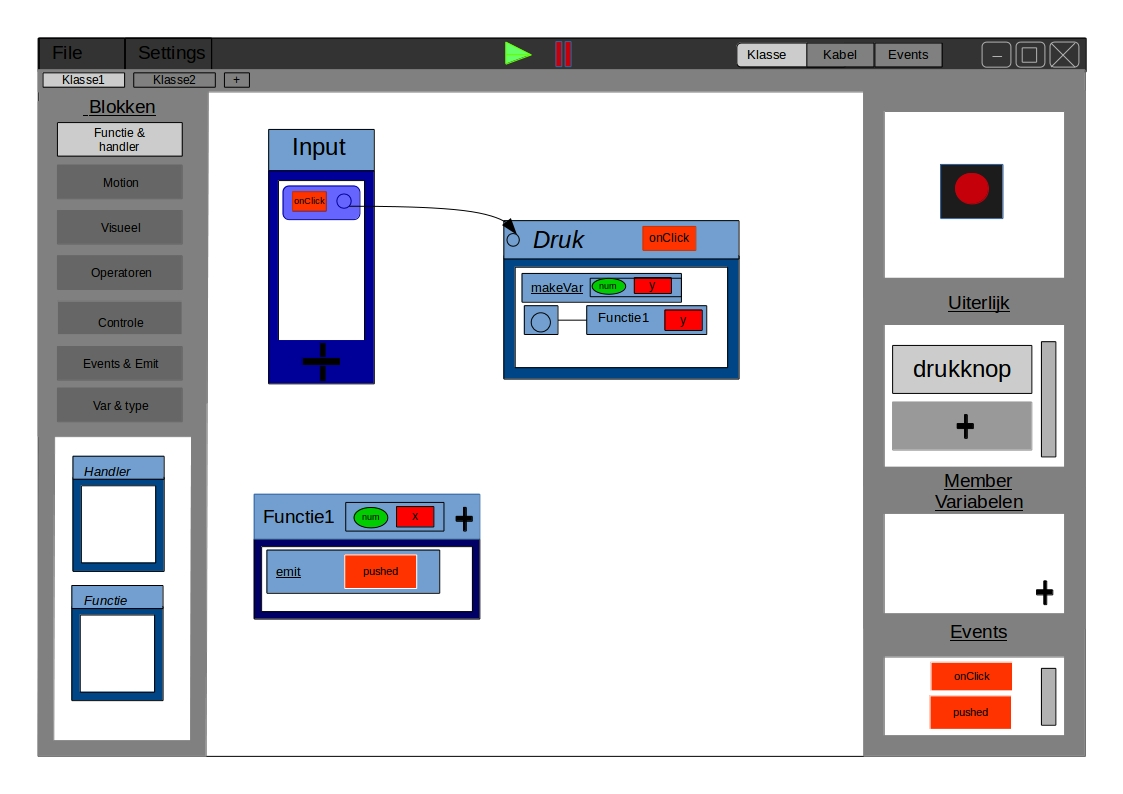
\includegraphics[scale=0.5]{../mockups/MockupCreatie.jpg}
  \caption{Mockup creatie klasse.}
  \label{creatieklassemockup}
\end{sidewaysfigure}
\clearpage
\subsection{Creatie instanties en kabels}
In dit view kan de gebruiker het hogere niveau van de werking van zijn programma definieren. De mockup van dit view is te zien op figuur \ref{wireframemockup}. Dit doet hij door instanties aan te maken van zijn eerder gedefineerde klassen. Hiervan heeft hij dan de keuze om de uitgaande events en inkomende event met elkaar te verbinden met behulp van pijlen. Hiermee kan hij beslissen aan welke instantie hij een event doorgeeft.\\ Bij een programma met veel kabels kan dit al snel voor een hele cluster zorgen. Daarom wordt er een filter voorzien waarmee de gebruiker kan bepalen van welke klasses hij geen kabels toont of welke event kabels hij niet toont.
\clearpage
 \begin{sidewaysfigure}
  \centering
   
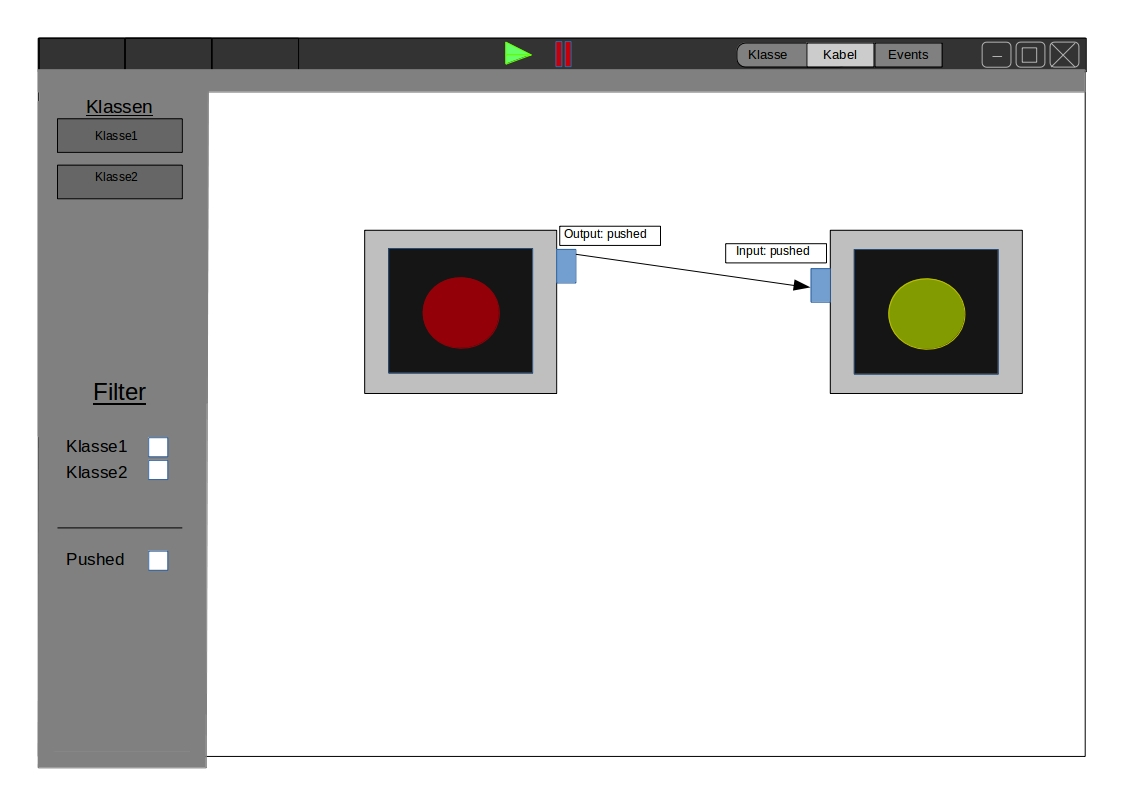
\includegraphics[scale=0.5]{../mockups/MockupWire.jpg}
  \caption{Mockup WireFrame.}
  \label{wireframemockup}
\end{sidewaysfigure}
\clearpage
\subsection{Event creatie}
In dit view kan de gebruiker een nieuw event defini\"{e}ren of een eerder gedefineerd event aanpassen. De mockup van dit view is te zien op figuur \ref{eventcreatiemockup}. Aan linkerkant van het venster bevindt er zich een overzicht van alle reeds gedefineerde events. Om een member aan het event toe te voegen gebruikt hij de plus knop en dan kan hij een member toevoegen van een gewenst type met een unieke naam. Een eerder toegevoegde member kan makkelijk verwijderd worden.
\clearpage
 \begin{sidewaysfigure}
  \centering
   
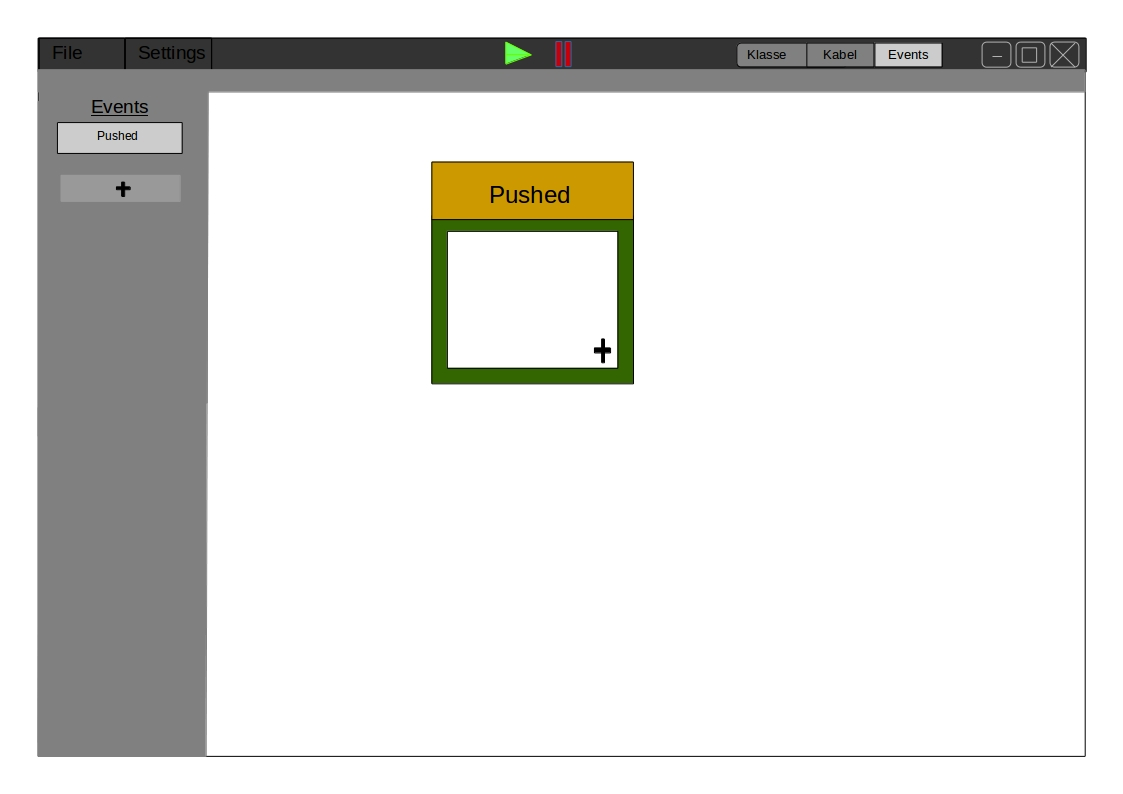
\includegraphics[scale=0.5]{../mockups/MockupsEvents.jpg}
  \caption{Mockup creatie event.}
  \label{eventcreatiemockup}
\end{sidewaysfigure}
\clearpage

\end{document}